\section{Taylorrreihen}
\begin{definition}{Definition Potenzreihen}
  \begin{centering}
  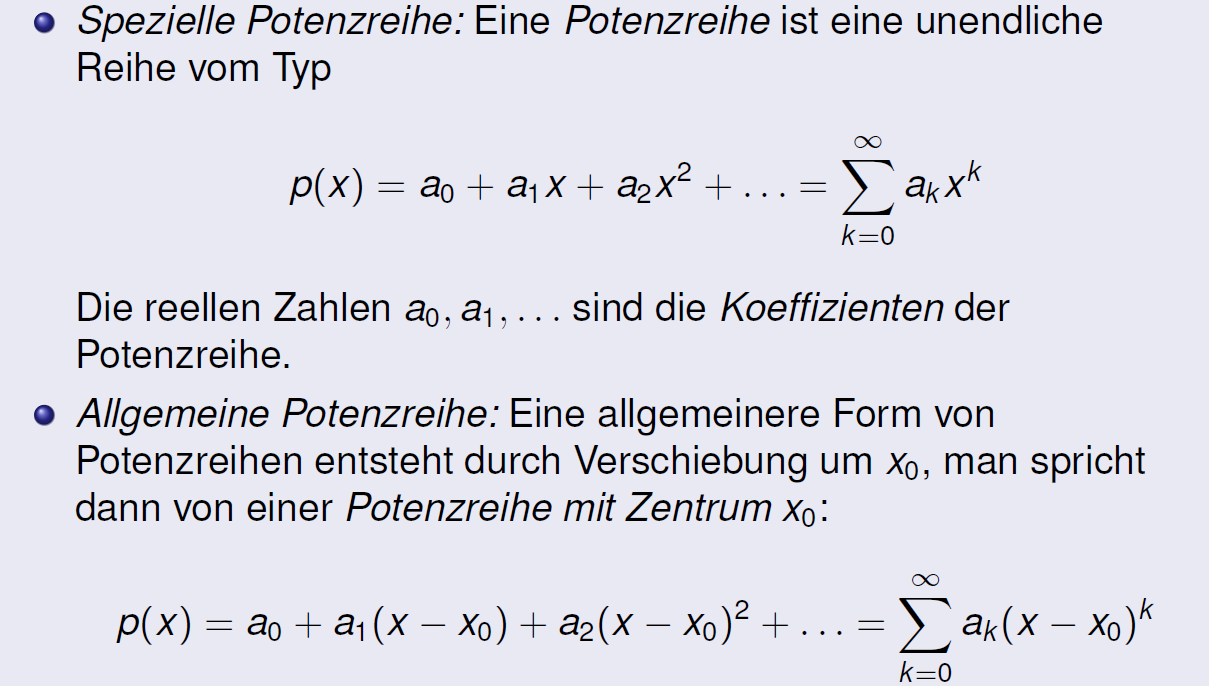
\includegraphics[width=0.8\textwidth]{images/2024-06-02-19-11-36.png}\\
  \end{centering}
\end{definition}
\begin{definition}{Definition Taylorreihe}\\
  \begin{centering}
  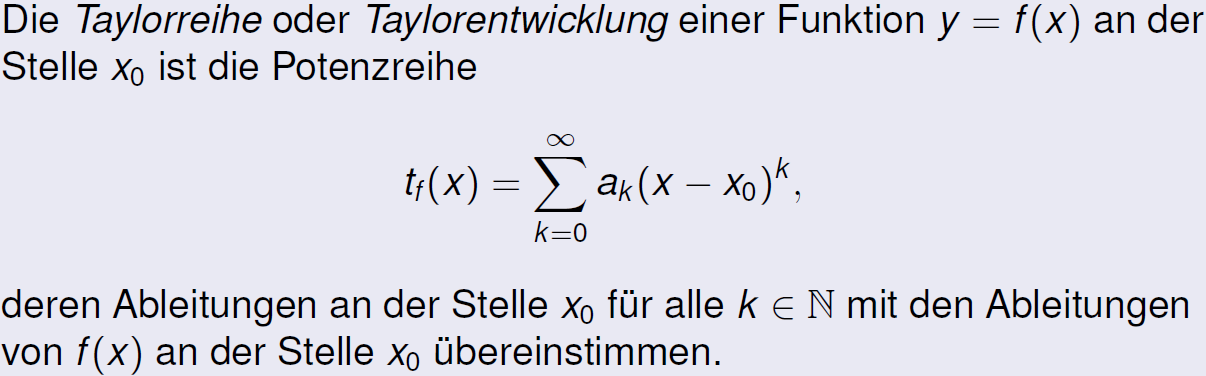
\includegraphics[width=0.8\textwidth]{images/2024-06-02-19-14-52.png}\\
  \end{centering}
\end{definition}
\begin{definition}{Definition Taylorpolynom}\\
  \begin{centering}
  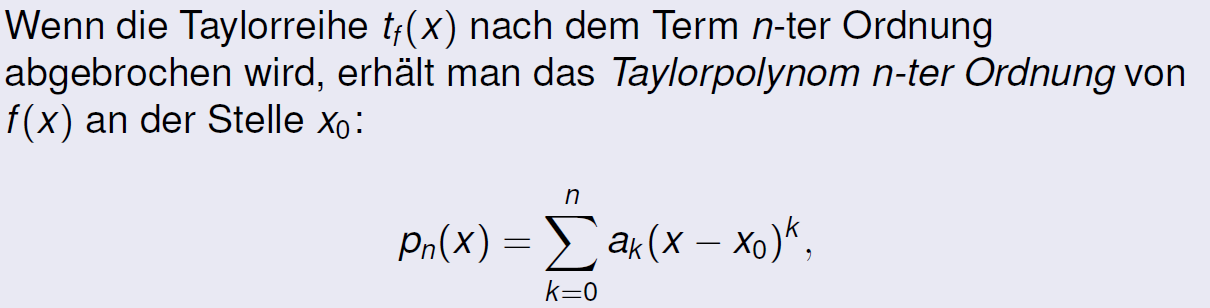
\includegraphics[width=0.8\textwidth]{images/2024-06-02-19-16-13.png}\\
  \end{centering}
  \begin{centering}
  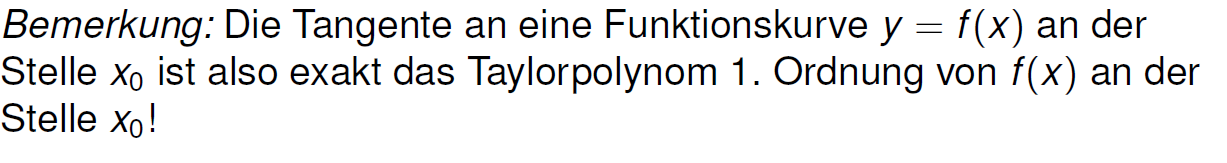
\includegraphics[width=0.8\textwidth]{images/2024-06-02-19-16-27.png}\\
  \end{centering}
\end{definition}
\begin{KR}{Vorgehen Berechnen Taylorreihe}\\
  \begin{centering}
  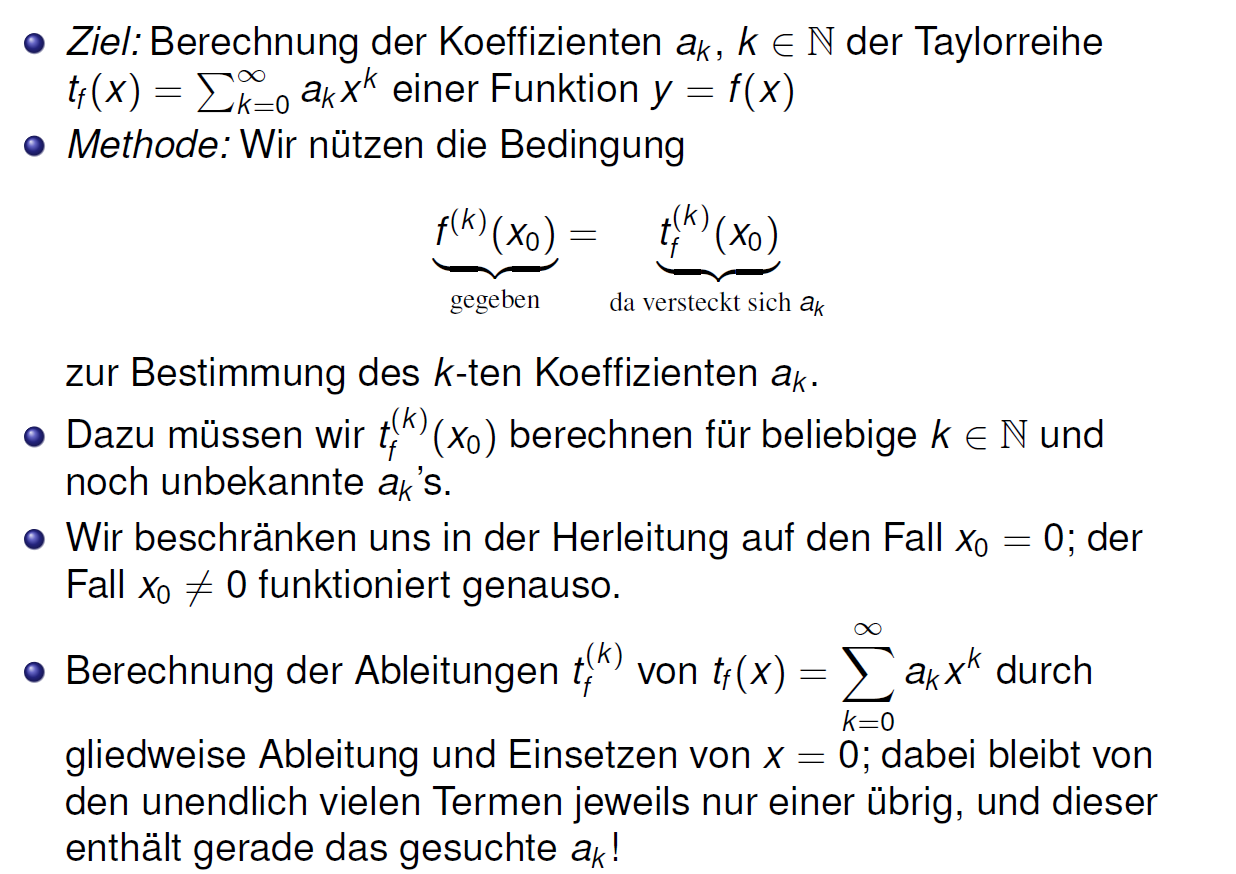
\includegraphics[width=0.8\textwidth]{images/2024-06-02-19-18-15.png}\\
  \end{centering}
\end{KR}
\begin{formula}{Formel für Taylorkoeffizienten}\\
  \begin{centering}
  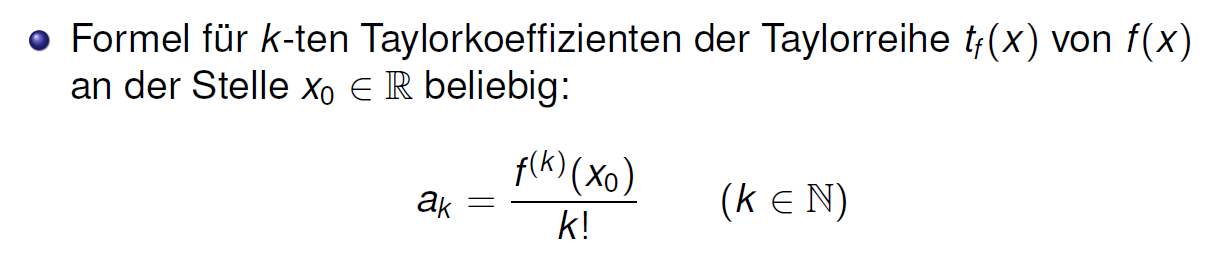
\includegraphics[width=0.8\textwidth]{images/2024-06-02-19-21-01.png}\\
  \end{centering}
  \begin{centering}
  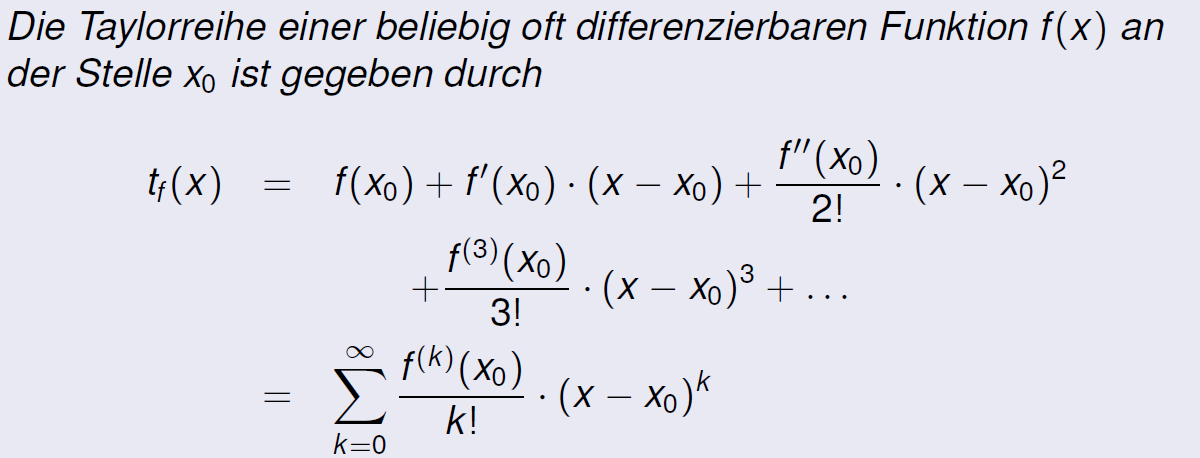
\includegraphics[width=0.8\textwidth]{images/2024-06-02-19-24-01.png}\\
  \end{centering}
\end{formula}
\subsection{Symetrie von Potenzreihen und Taylorreihen}
\begin{lemma}{Symetrie von Funktionen}\\
  \begin{centering}
    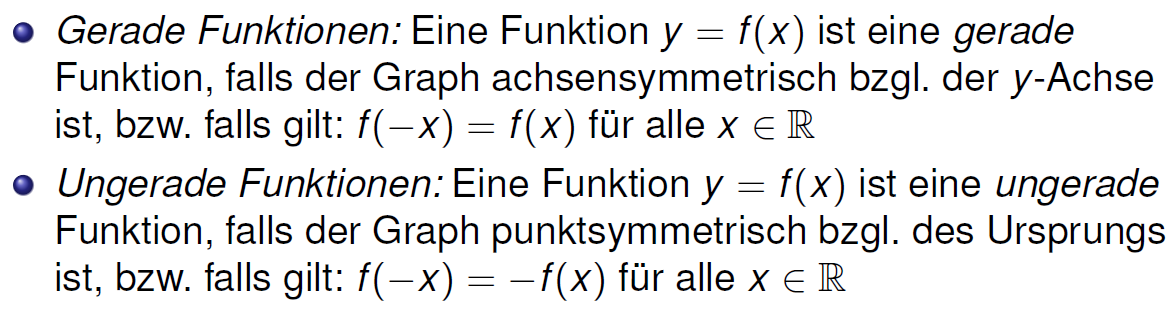
\includegraphics[width=0.8\textwidth]{images/2024-06-02-19-25-55.png}\\
  \end{centering}
\end{lemma}
\begin{lemma}{Symetrie von Potenzreihen}\\
  \begin{centering}
  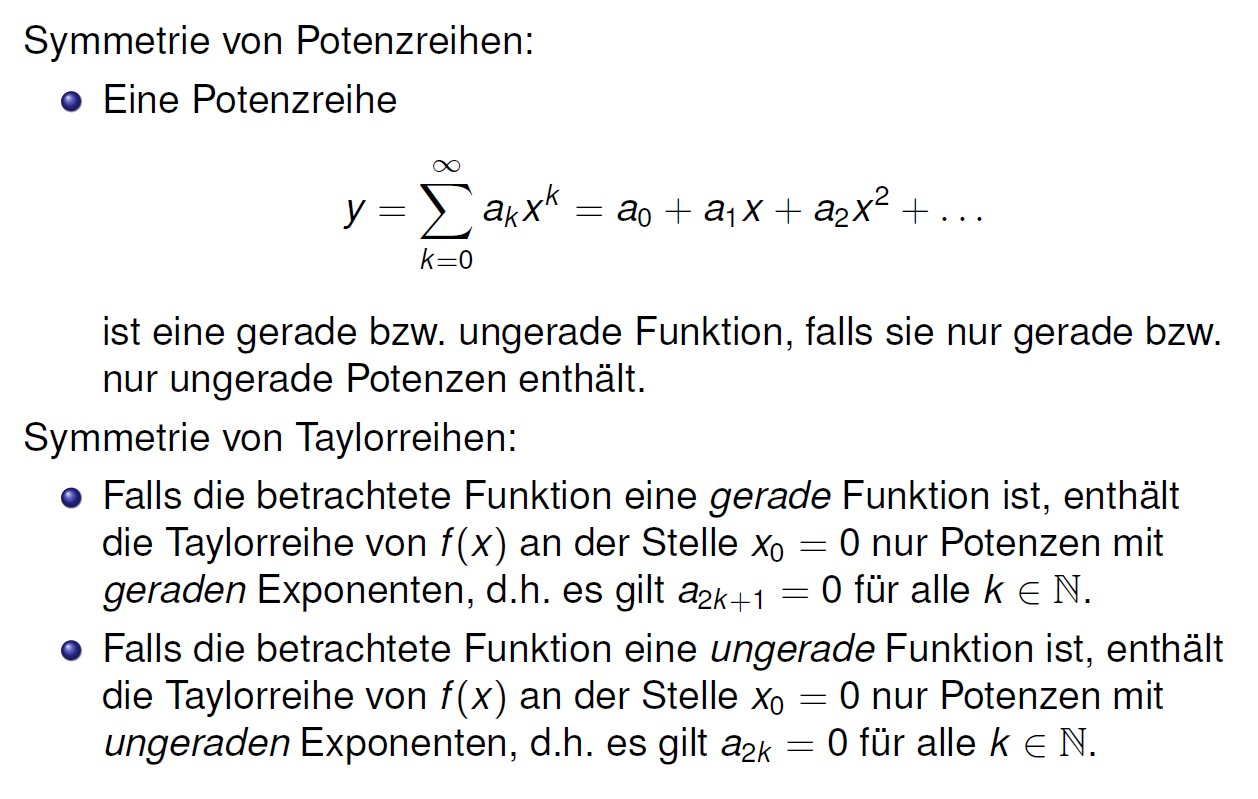
\includegraphics[width=0.8\textwidth]{images/2024-06-02-19-28-18.png}\\
  \end{centering}
\end{lemma}
\begin{lemma}{Binomialkoeffizienten}\\
  \begin{centering}
  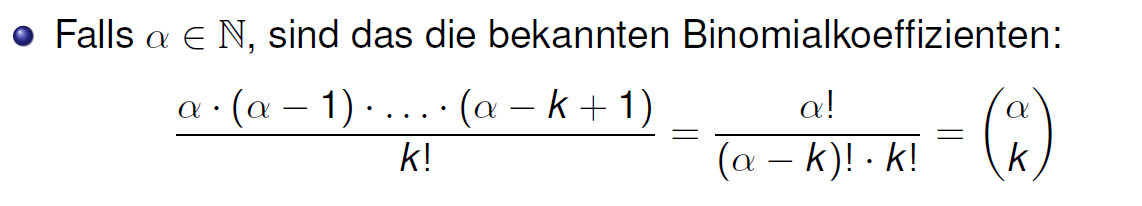
\includegraphics[width=0.8\textwidth]{images/2024-06-02-19-31-35.png}\\
  \end{centering}
  \begin{centering}
  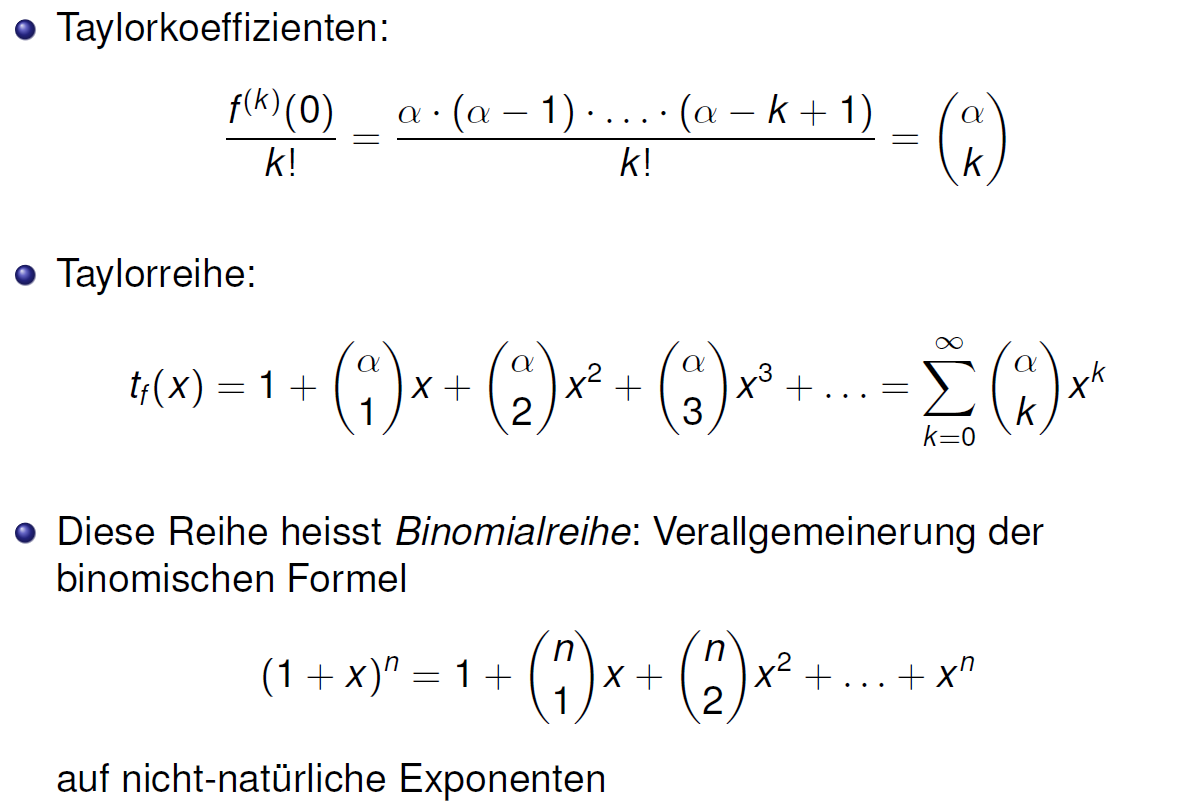
\includegraphics[width=0.8\textwidth]{images/2024-06-02-19-32-15.png}\\
  \end{centering}
\end{lemma}
\begin{definition}{Regel von Bernoulli- de l’Hospital}\\
  \begin{centering}
  
\includegraphics[width=0.8\textwidth]{images/2024-06-02-21-42-08.png}\\
  \end{centering}
  \begin{centering}
  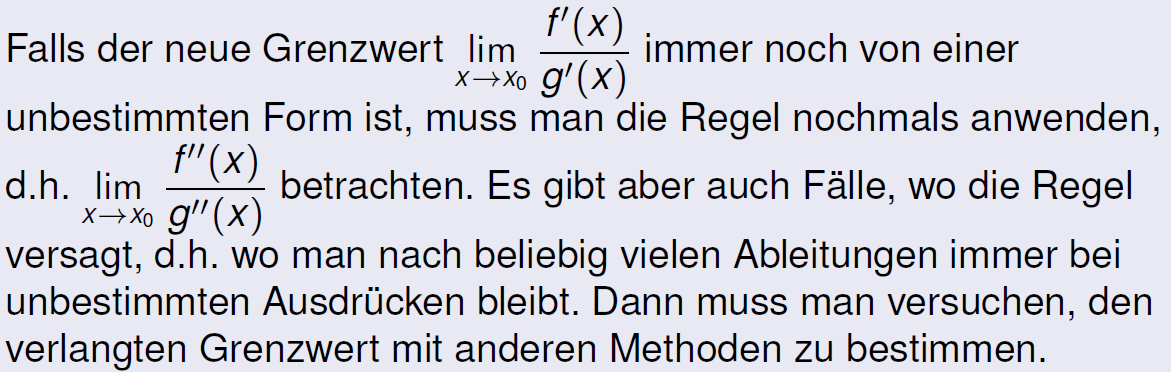
\includegraphics[width=0.8\textwidth]{images/2024-06-02-21-42-41.png}\\
  \end{centering}
\end{definition}
\begin{definition}{Varianten von l'Hospital}\\
  \begin{centering}
  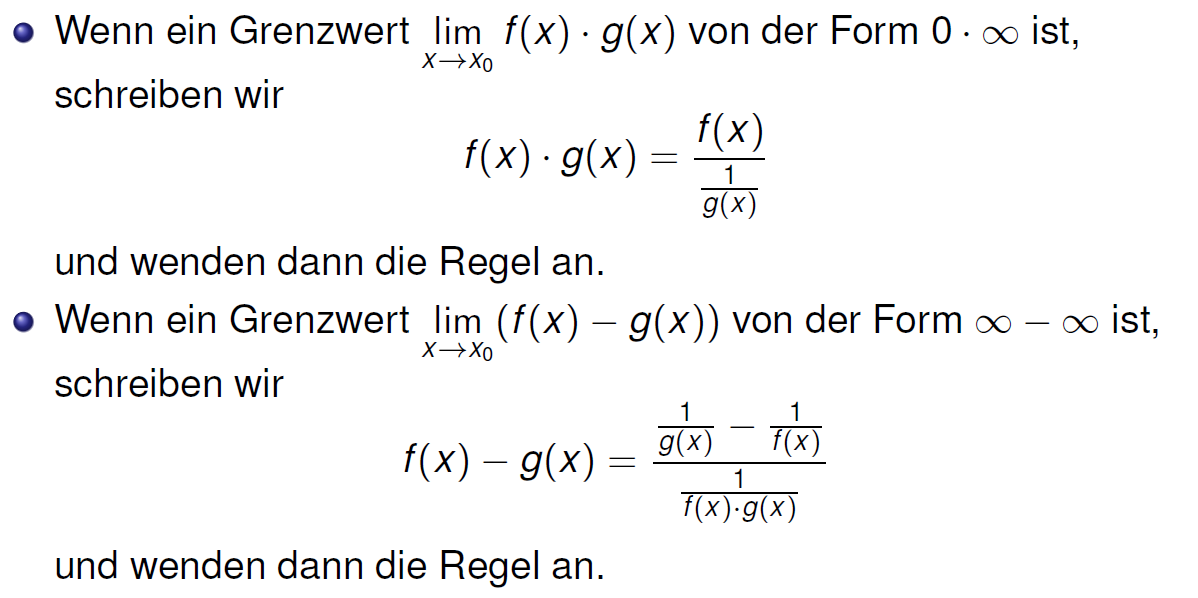
\includegraphics[width=0.8\textwidth]{images/2024-06-02-21-43-36.png}\\
  \end{centering}
\end{definition}
\begin{definition}{Genauigkeit der Approximation}\\
  \begin{centering}
  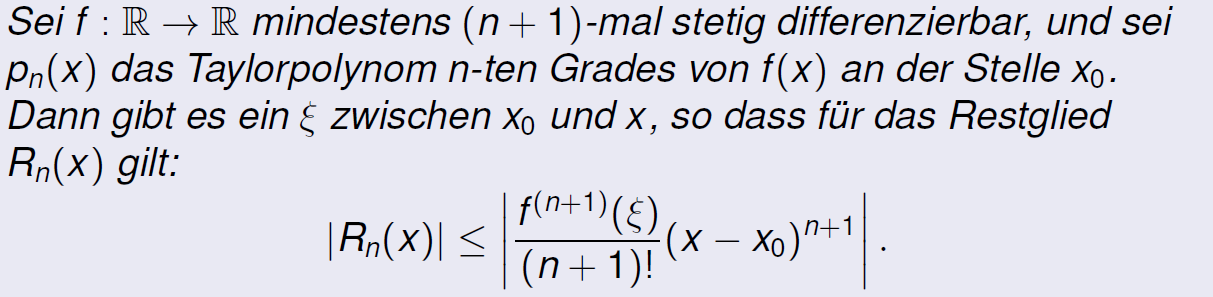
\includegraphics[width=0.8\textwidth]{images/2024-06-02-21-45-47.png}\\
  \end{centering}
\end{definition}
\subsection{Konvergenz von Potenzreihen}
\begin{definition}{Konvergenzradius}\\
  \begin{centering}
  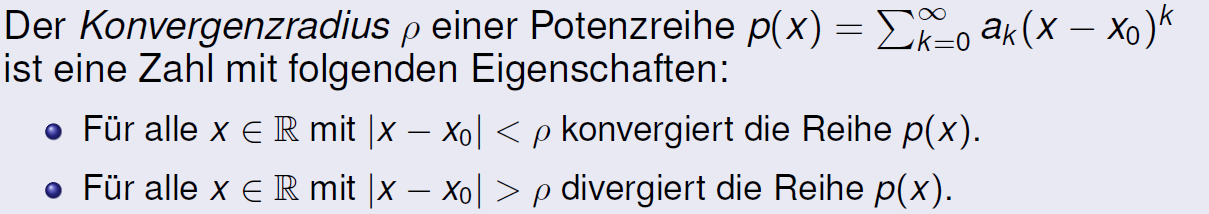
\includegraphics[width=0.8\textwidth]{images/2024-06-02-21-48-37.png}\\
  \end{centering}
  \begin{centering}
  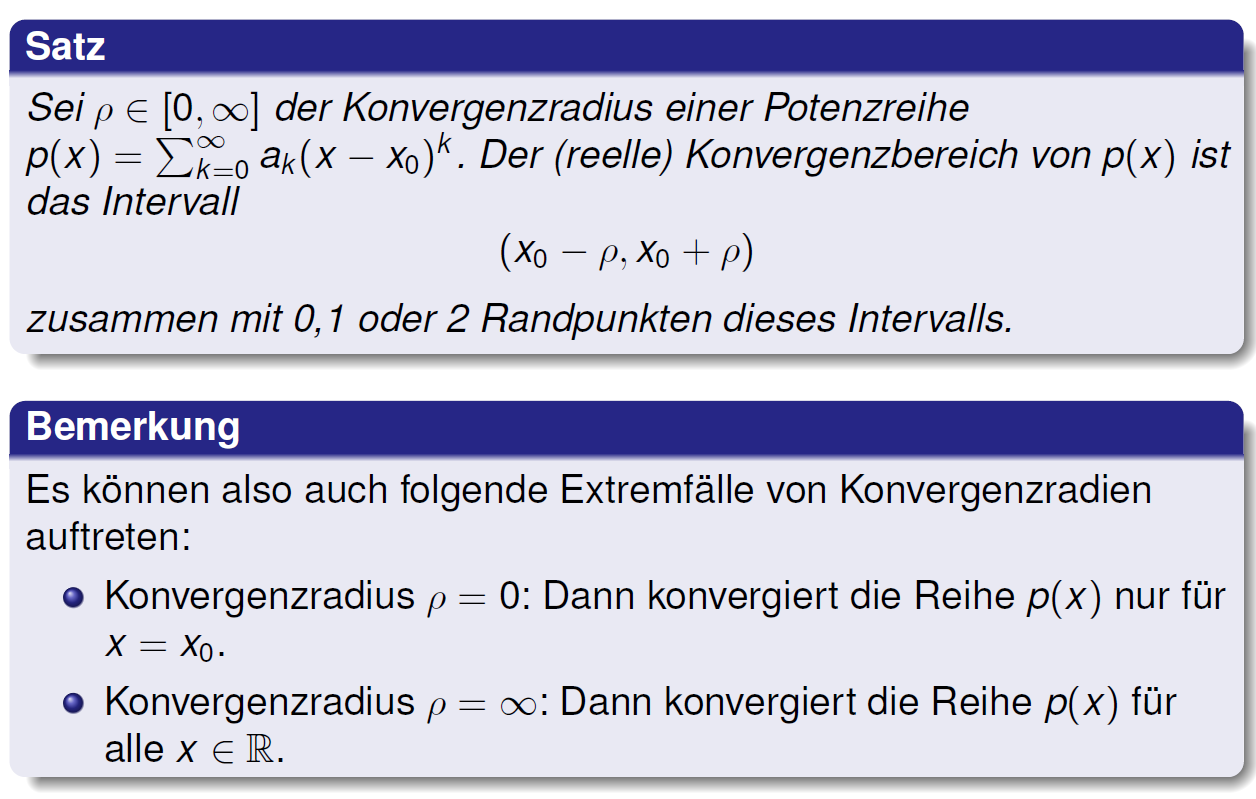
\includegraphics[width=0.8\textwidth]{images/2024-06-02-21-53-30.png}\\
  \end{centering}
\end{definition}
\begin{formula}{Konvergenzradius Formel}
  \begin{centering}
  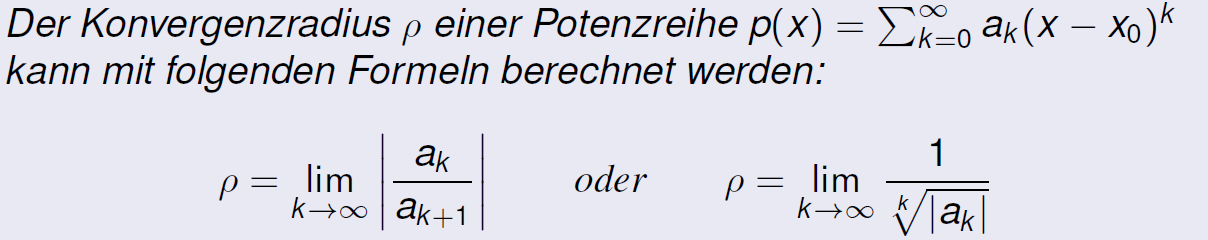
\includegraphics[width=0.8\textwidth]{images/2024-06-02-21-54-17.png}\\
  \end{centering}
\end{formula}
